\documentclass{article}
\usepackage{amsmath}
\usepackage{optidef}
\usepackage{amssymb}
\usepackage[utf8x]{inputenc}
\usepackage{graphicx}
\usepackage[]{algorithm2e}
\graphicspath{ {rsc/} }
\allowdisplaybreaks
\title{Rapport technique}
\author{
	AGUSTO Rold 
	\and 
	PAUL Hugo 
	\and 
	TRANG Hoang Phong Vu
	\and 
	SUGANATHASIVAM Vathanalakshan
	}
	
\begin{document}
\maketitle
\section{Intoduction}
TODO : Introduction
\section{Problème du voyageur de commerce déterministe}
Afin de pouvoir traiter le problème du voyageur de commerce stochastique, nous partons de l'origine avec l'approche déterministe. Dans cette approche, les distances entre les villes sont connues avant que le commerçant commence le voyage.  Plus concrètement, soit:\\
\begin{itemize}
\item G = (V, E) un graphe orienté ou non-orienté complet avec :
		\begin{itemize}
			\item V un ensemble de sommets
			\item \( E \subseteq \{(x, y) | (x, y) \in V^2 \wedge x \neq y \} \) un ensemble d'arêtes, qui sont des couples de sommets distincts
		\end{itemize}
\item \(c_{ij}\) le coût pour aller du sommet \(v_{i}\) au sommet \(v_{j}\)
\item \(x_{ij}\) la variable de décision. elle vaut 1 s'il existe un arc \((v_{i}, v_{j})\), 0 sinon. On peut l'interpréter comme une matrice de passage.
\end{itemize}
Le problème du voyageur de commerce peut être écrit sous forme problème d'optimisation :
\begin{mini!}|s|[1]                   % mini! = minimize 
    {x}                               % optimization variable
    {\sum_{i=1}^{n}\sum_{j=1}^{n}c_{ij}x_{ij}\label{eq:optd}}   % objective function and label
    {\label{eq:Example1}}             % label for optimization problem
    {}                                % optimization result
    \addConstraint{\sum_{j=1, i \neq j}^{n} x_{ij}}{= 1, \quad & i = 1,...  \label{eq:optd_con1}}
    \addConstraint{\sum_{i=1, i \neq j}^{n} x_{ij}}{= 1, \quad & j = 1,...  \label{eq:optd_con2}}   
    \addConstraint{\sum_{i|v_i \in S} \sum_{j|v_j \in S}x_{ij}} {\leq |S| - 1 \quad & S \subset V \textrm{et} S \neq \varnothing \label{eq:optd_con3}}
    \addConstraint{x_{ij} } {\in \{0, 1\} \quad & 1 \leq i, j \leq n \label{eq:optd_con4}}
\end{mini!}
Littéralement, le voyageur doit visiter toutes les villes (connues dans le graphe) tel que la distance qu'il parcourt est minimale et que pour chaque ville il ne peut visiter qu'une seule fois. Plus concrètement, la fonction objectif sert à trouver la distance minimale. La contrainte \ref{eq:optd_con1} veut dire : après avoir visté une ville \(v_i\), le voyageur ne peut visiter qu'une ville ensuite. Avec la contrainte \ref{eq:optd_con2}, lors d'une visite d'une ville \(v_j\), le voyageur doit provenir d'une seule ville. \\En comparant avec les conditions littérales qu'on a prises en compte précédémment, les deux premières contraintes sont suffisantes. Néanmoins, les algorithmes d'optimisation des solveurs peuvent génerer des subtours (i.e. sous chemins). Toutes les villes sont visitées une seule fois et la distance totale est minimale, mais le fait d'avoir plusieurs chemins discrètes veut dire que le voyageur a le droit de téléporter d'une ville en une autre ville et ce n'est pas le cas. La contrainte (\ref{eq:optd_con3}) est donc rajoutée au modèle pour les éliminer, elle est appelée la contrainte d'élimination des subtours.\\

\begin{figure}[h]\centering
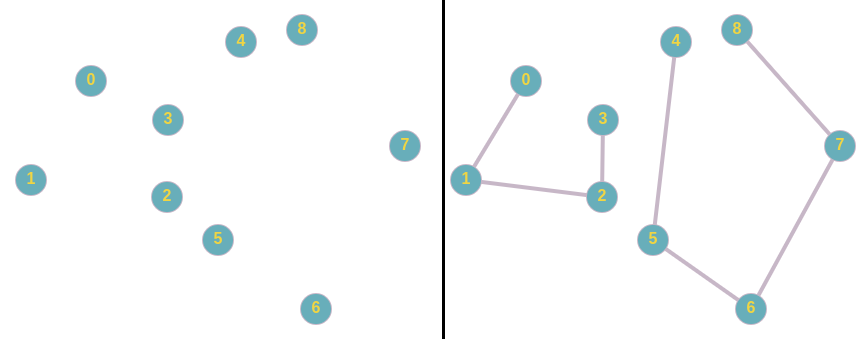
\includegraphics[width=0.5\textwidth]{graphe_avec_subtour}
\caption{Une solution où existe plusieurs subtours (sous-chemins) (Attention, il s'agit d'un exemple pour montrer la conséquence d'une manque de la contrainte \ref{eq:optd_con4}, elle n'est donc pas une solution optimale)}

\end{figure}
Une approche possible pour ce modèle est de lancer l'optimisation avec les contraintes (\ref{eq:optd_con1}), (\ref{eq:optd_con2}), (\ref{eq:optd_con4}) plusieurs fois jusqu'à ce qu'on obtient la solution optimale. La démarche est exprimée dans le pseudo-code ci-dessous :\\
\begin{algorithm}[H] 
 \KwData{graphe G=(V, E)}
 \KwResult{La solution optimale du problème du voyageur de commerce}
   nS \(\leftarrow +\infty\)  \;
 \While{nS n'est pas optimale}{
  lancer l'optimisation avec les contraintes \ref{eq:optd_con1} \ref{eq:optd_con2} \ref{eq:optd_con4}\;
  nS \(\leftarrow\) nombre de sous graphes de l'optimisation\;
 }
 \caption{Trouver la solution optimale du problème du voyageur de commerce}
\end{algorithm}
En effet, pour la contrainte d'élimination de subtours, il existe plusieures formulations possibles. Dans le cadre de notre projet, on a décidé d'utiliser celle de Miller-Tucker-Zemlin pour des raisons de simplicité et efficacité:
\begin{equation}
\begin{aligned}
	u_i - u_j + nx_{ij} \leq n - 1, \quad & 2 \leq i \neq j \leq n \\
	1 \leq u_j \leq n - 1, \quad & 2 \leq i \leq n
\end{aligned}
\end{equation}
La variable \(u_i \in \mathbb{N} \cup \{0\}\) est une variable de décision, elle indique l'ordre de passage de la ville i. De ce fait, \(u_i \leq u_j\) implique que la ville i est visité avant la ville j.\\
TODO : montrer la solution\\
\section{Problème du voyageur de commerce stochastique}
Nous avons traité le problème du voyageur de commerce de façon exacte où les coûts (i.e les distance, la durée, etc.) sont connus dans la partie précédente. Dans cette partie, on considère que ces coûts ne sont plus exacts mais aléatoires. C'est-à-dire qu'ils suivent chacun une loi de probabilité. On suppose que les coûts \(\tilde{c}\) sont des variables aléatoires qui suivent une distribution normale dont la moyenne est \(\bar{c}\) et la matrice de variance-covariance est \(\sum\) : \(\tilde{c_{ij}} \sim \mathcal{N}(\bar{c_{ij}},\,\sigma_{ij}^{2})\,. \).\\
Le modèle mathématique devient donc :
\begin{mini!}|s|[2]                   % mini! = minimize 
    {x}                               % optimization variable
    {\sum_{i=1}^{n}\sum_{j=1}^{n}\bar{c_{ij}}x_{ij}\label{eq:opts}}   % objective function and label
    {\label{eq:Example1}}             % label for optimization problem
    {}                                % optimization result
    \addConstraint{\sum_{j=1, i \neq j}^{n} x_{ij}}{= 1, \quad & i = 1,...  \label{eq:opts_con1}}
    \addConstraint{\sum_{i=1, i \neq j}^{n} x_{ij}}{= 1, \quad & j = 1,...  \label{eq:opts_con2}}   
    \addConstraint{\sum_{i|v_i \in S} \sum_{j|v_j \in S}x_{ij}} {\leq |S| - 1 \quad & S \subset V \textrm{et} S \neq \varnothing \label{eq:opts_con3}}
    \addConstraint{P ( \sum_{i=1}^{n}\sum_{j=1}^{n}\tilde{c_{ij}}x_{ij} \leq Z) \geq \alpha \label{eq:opts_con4}}
    \addConstraint{x_{ij} } {\in \{0, 1\} \quad & 1 \leq i, j \leq n \label{eq:opts_con5}}
\end{mini!}
La contrainte (\ref{eq:opts_con4}) a été rajoutée dans ce modèle. Elle est appelée contrainte en probabilité. Elle modélise le risque pris par le voyageur de commerce, et doit être satisfaite dans au moins de \(\alpha\%\) des cas. La constante Z est la valeur de la solution optimale du problème déterministe majorée de 20 à 30\%.\\
On peut voir que ce n'est pas possible d'implémenter directement la contrainte en probabilité (\ref{eq:opts_con4}) en CPLEX. Il faut donc transformer la probabilité en une autre forme.\\
Plus concrètement:\\
\begin{equation}
\begin{aligned}
\textrm{On a : } 
& \tilde{c_{ij}} \sim \mathcal{N}(\bar{c_{ij}},\,\sigma_{ij}^{2})\\
&\Rightarrow x_{ij}\tilde{c_{ij}} \sim \mathcal{N}(x_{ij}\bar{c_{ij}},\, x_{ij}^2\sigma_{ij}^{2})\\
&\Rightarrow \sum_{i}^n \sum_{j}^n x_{ij}\tilde{c_{ij}} \sim \mathcal{N}(\sum_{i}^n \sum_{j}^n x_{ij} x_{ij}\bar{c_{ij}},\, \sum_{i}^n \sum_{j}^n x_{ij} x_{ij}^2\sigma_{ij}^{2})\\
&\textrm{Appelons } X = \sum_{i}^n \sum_{j}^n x_{ij}\tilde{c_{ij}}\\ 
&\Rightarrow X \sim \mathcal{N}(\sum_{i}^n \sum_{j}^n x_{ij} x_{ij}\bar{c_{ij}},\, \sum_{i}^n \sum_{j}^n x_{ij} x_{ij}^2\sigma_{ij}^{2})\\
\textrm{(\ref{eq:opts_con4}) devient :} 
& P(X \leq Z) \geq \alpha \\
&\Leftrightarrow F_X(Z) \geq \alpha\\
&\Leftrightarrow Z \geq F_X^{-1}(\alpha) \textrm{ ou } F_X^{-1}(\alpha) \leq Z\\
&\Leftrightarrow \sum_i^n \sum_j^n \bar{c_{ij}} x_{ij} + \sum_i^n \sum_j^n x_{ij} \sigma_{ij} \sqrt{2}erf^{-1}(2\alpha - 1) \leq Z\\
&\Leftrightarrow \sum_i^n \sum_j^n x_{ij}  (\bar{c_{ij}}  + \sigma_{ij} \sqrt{2}erf^{-1}(2\alpha - 1)) \leq Z\\
&\Leftrightarrow \sum_i^n \sum_j^n x_{ij} \Phi^{-1}(\alpha) \leq Z \\
\textrm{Alors, (\ref{eq:opts_con4}) devient } & \sum_i^n \sum_j^n x_{ij} \Phi^{-1}(\alpha) \leq Z \label{eq:opts_con4q}\\
\end{aligned}
\end{equation}\\
\(\Phi^{-1}\) est la fonction quantile de la loi Normale \(\mathcal{N}(\bar{c_{ij}},\,\sigma_{ij}^{2})\), ou simplement l'inverse de la fonction cummulative \(F_{\tilde{c_{ij}}}(Z)\).\\
Dans le cadre de ce projet, on considère que la moyenne de ses lois normales sont des coûts donnés dans les fichiers *.TSP fournit par la librairie TSPLIB. Il nous reste donc à déterminer ces variances. Nous proposons de les générer de façon aléatoire pour chaque coût \(\tilde{c_{ij}}\) donné.
Enfin, comme expliqué ci-dessus, Z est la solution du problème du voyageur de commerce, majorée de 20 à 30\%, il faut donc d'abord obtenir la solution du problème déterministe. Ensuite, il ne reste qu'à lancer la résolution avec la contrainte (\ref{eq:opts_con4})
\end{document}